\documentclass{article}
\usepackage{tikz}
\usepackage[top=2cm, bottom=2cm, outer=0cm, inner=0cm]{geometry}
\usepackage[absolute,overlay]{textpos}
  \setlength{\TPHorizModule}{1mm}
  \setlength{\TPVertModule}{1mm}
\begin{document}
\tikz[remember picture,overlay] \node[opacity=0.2,inner sep=0pt] at (current page.center){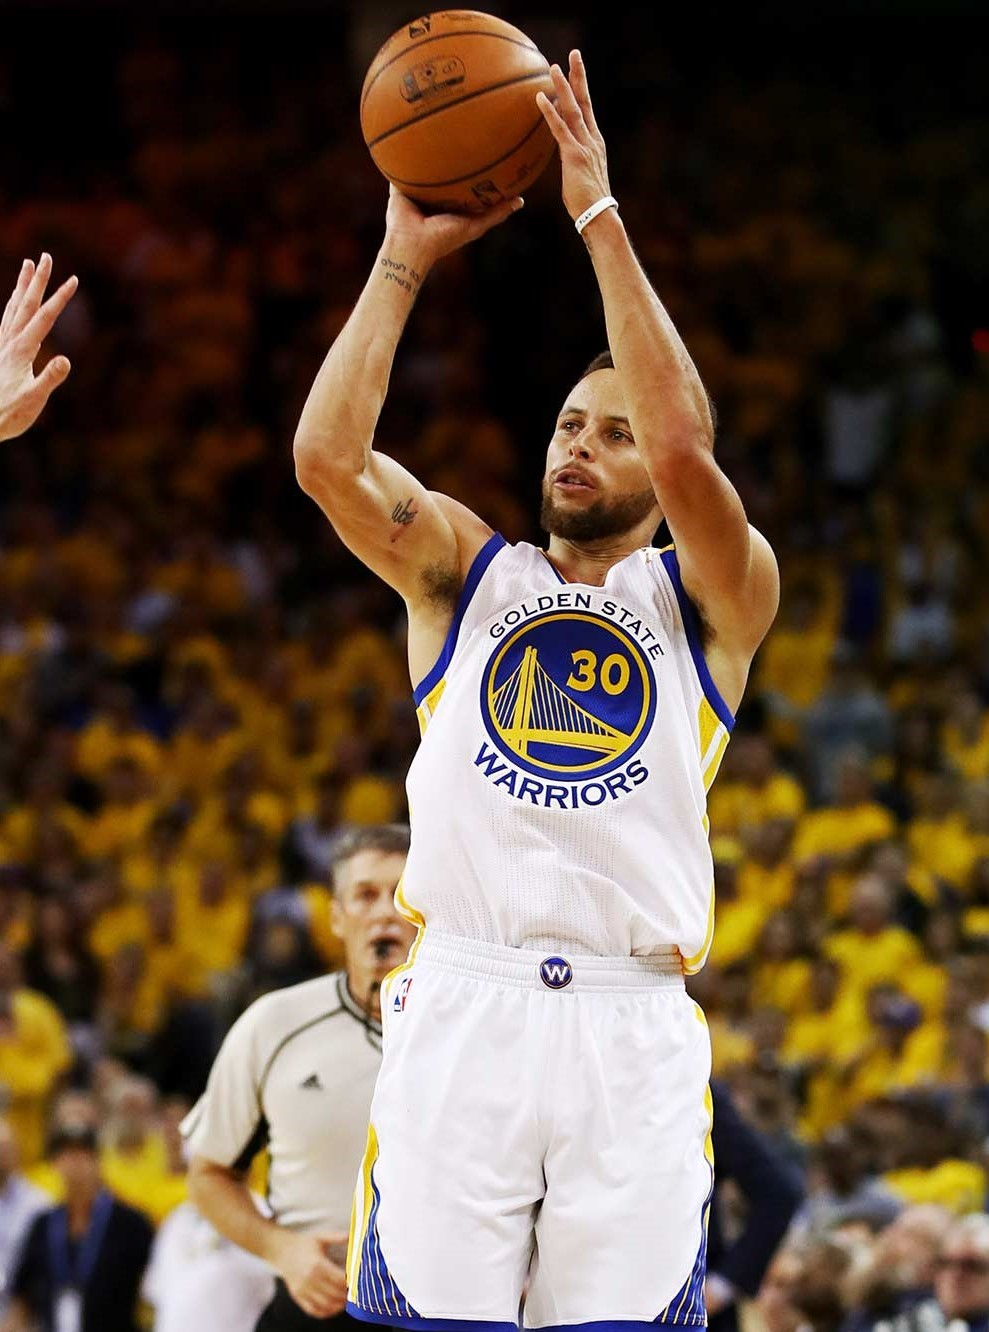
\includegraphics[width=\paperwidth,height=\paperheight]{steph.jpg}};
\begin{center}
 {\huge \bf The Significance of 3-Point Shooting in the NBA Draft}
 
 \vspace{0.1in}
 %by Tim Krumwiede, Ph.D.
\end{center}


\begin{textblock}{80}(0,40)
      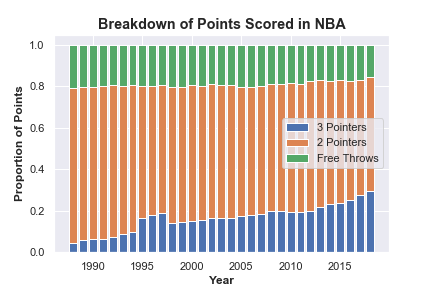
\includegraphics[width=\linewidth]{pts_breakdown.png}
    \end{textblock}
    
\begin{textblock}{60}(0,95)
      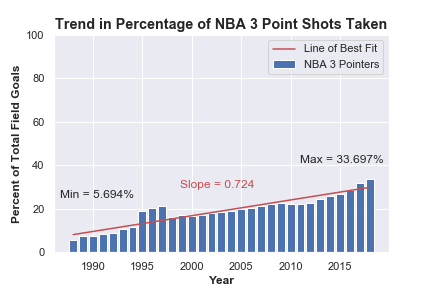
\includegraphics[width=\linewidth]{3pt_taken_nba.png}
    \end{textblock}
    
\begin{textblock}{60}(0,135)
      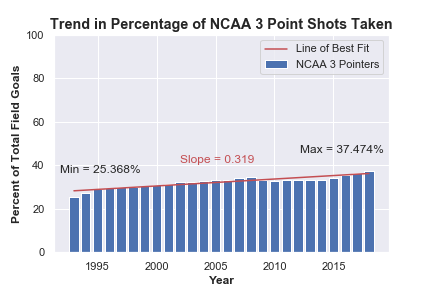
\includegraphics[width=\linewidth]{3pt_taken_ncaa.png}
    \end{textblock}
    
\begin{textblock}{60}(0,175)
      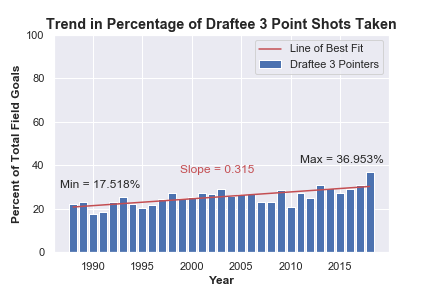
\includegraphics[width=\linewidth]{3pt_taken_df.png}
    \end{textblock}
    
\begin{textblock}{75}(0,215)
      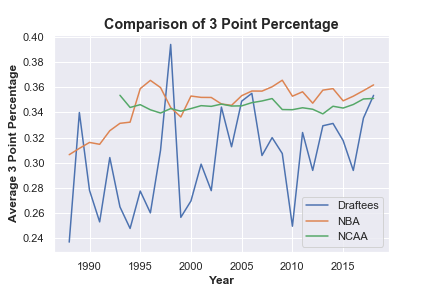
\includegraphics[width=\linewidth]{3pt_comp.png}
    \end{textblock}
    
\begin{textblock}{75}(70,215)
      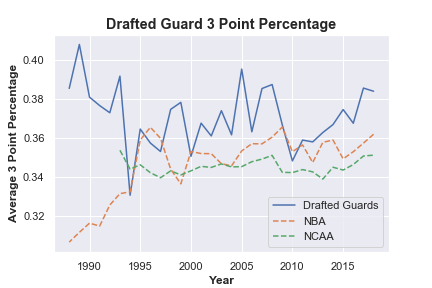
\includegraphics[width=\linewidth]{3pt_g.png}
    \end{textblock}

\begin{textblock}{75}(140,215)
      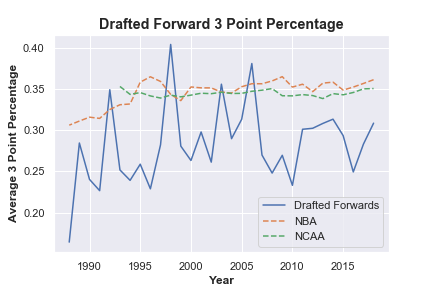
\includegraphics[width=\linewidth]{3pt_f.png}
    \end{textblock}
   
   
\begin{textblock}{120}(85,55)
{\bf How important is 3-point shooting to NBA teams when drafting players out of college?}

\vspace{0.1in}
     The NBA introduced the three-point shot, shots from farther than 23 feet and 9 inches from the basket that count for three points instead of two, in the 1979-80 season. The shot has become increasingly more important as more and more of the total points scored are produced by three pointers. This is clear in the graph to the left, in which the percentage of points from three pointers has risen steadily (with the exception of three seasons from 1994 to 1997 in which the three-point line was changed to only 22 feet from the basket).
         \end{textblock}  
         
         

\begin{textblock}{135}(70,105)  
     It is then no surprise that players are taking more and more three pointers. The amount of three pointers taken as a percentage of total shots in the NBA is shown to the left. Compare this graph with those below it, depicting the analagous data for the NCAA and drafted college players that later played in the NBA. 
     
     The percentage of 3 pointers taken in the NBA has increased at an average rate of 0.724 percentage points per year. In contrast, the number of three pointers taken by players in the NCAA is less than those that of the NBA, but with a shallower slope. The fact that the three-point line in the NCAA is 3 feet closer to the basket is almost certainly the primary reason for this. The next graph to the left is the percentage of three-pointers taken by drafted players from the project dataset in their last year in college. The variance is much higher than the NCAA graph due to being a smaller sample, but there does not appear to be any significant difference in either magnitude or slope. This seems to suggest that overall, NBA prospects have not taken more three-pointers than the NCAA average.
     
     \vspace{0.1in}
     A player's three-point shooting abililty is always measured by three-point percentage: shots made divided by attempts. Let's take a look at how NBA prospects in our dataset compare to both NBA and NCAA averages. At bottom left, we see that while draftees' percentage varies greatly from year to year, it is almost always below both league averages. Perhaps it is more useful to examine this by position: guards typically shoot the most threes, forwards often shoot threes, and centers very rarely shoot threes.
     Bottom center we see that drafted guards are mostly above both league averages,  but perhaps surprisingly there does not appear to be an upward trend despite how three pointers have increased in importance. The same goes for forwards in the bottom right graph, although the shoot less than league averages.
    \end{textblock}  
    
\end{document}